\chapter{Aim of the Work}

As we discussed in Chapter \ref{chap:introduciton}, metamorphic
self-reconfigurable robots have several properties which makes them an appealing
direction for future robotics trends. Those include versatility, fast
prototyping and high-level of fault-tolerance. However, in the current state of
the art we are far away from reaching these properties in practice. As we showed
in Chapter \ref{chap:state-of-the-art}, the research in this area is broad and
vivid. Yet, there are plenty of challenges and open-problems to tackle.

From all the challenges that metamorphic robots present, I would like to focus
on finding ways to control metamorphic robots in fault-tolerant manner via
distributed control in my research. I further describe my goals in the following
text.

\section{Evaluation Platform}

I would like to demonstrate the solutions I will propose on a physical robots. I
would also like to make my research as reproducible as possible. That is
unfortunately quite hard in the area of robotics as one cannot easily download a
robot and test my solutions.

To achieve the best reproducibility as possible, it is crucial to use a hardware
platform which is easily obtainable. As we addressed in section
\ref{sec:reproducibility}, none of the platforms we discussed in chapter
\ref{chap:state-of-the-art} has manufacturing data (for mechanical construction
and PCBs) nor firmware publicly available. We also contacted the authors if they
are willing to share their design files or if there is a possibility to buy
their robots. Unfortunately none of them responded positively. Only the authors
of SMORES \cite{DBLP:conf/iros/DaveyKY12} responded that it would be possible to
cooperate and try our solutions on their robots at their facility, which is not
convenient.

Therefore, as a by-product of my PhD study I would like to develop an
open-hardware and open-source platform for metamorphic distributed robots. This
platform should serve as tool for demonstration of my research outcomes which
allows the others to easily build their own robots and reproduce my results.
Also, by being the first open platform, it should serve as a research tool for
the others in the area.

The platform, called the RoFI platform, is part of my study I have advanced the
most so far and we introduce more in detail in Chapter \ref{chap:results}.

\section{Fault Tolerant Distributed Control for RoFI}

In my research I would like omit the reconfiguration part from the control and
mainly mainly focus on designing fault-tolerant controllers that perform given
task without changing the robot shape. I would like to propose controllers that
are distributed since they should offer more feasible path towards fault
tolerance compared to centralized approaches.

I would like to focus on a partial module malfunction, since
system explosion is more related to research about spatial localization and path
planning than distributed control. Similarly, complete module malfunction is
probably better solved by reconfiguration as distributed control has no other
option to deal with a completely malfunctioned module than to ignore it.

A robot without sensors cannot interact with the environment and can only follow
hard-coded paths and therefore, can be used only a highly controlled
environment. This is contrary to the overall motivation for metamorphic robots,
therefore these robots have to feature a large number of sensor. In practice,
one can expect that some of this sensors can report faulty readings or become
faulty. Similarly, with large number of communicating nodes, we can expect
communication errors to be present. Therefore, I would like more specifically
propose a solution for controlling metamorphic systems where the individual
modules can feature Byzantine faults originating from their sensors or faulty
communication.

\section{Proposed Case Studies}

During my PhD study I would like to perform two case studies to tackle the
challenges I stated above. That is to design a distributed controllers for
specific configurations, which allow the system to transport in space and be
fault tolerant for partial module failures. After performing those case
studies, I would like to generalize the findings and to introduce a more general
approaches if applicable.

\begin{figure}[!t]
    \centering
    \begin{subfigure}[b]{0.45\textwidth}
        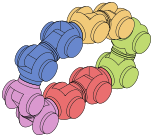
\includegraphics[width=\textwidth]{figures/ring_example.pdf}
        \caption{Loop Robot}
        \label{fig:example_roller}
    \end{subfigure}
    ~
    \begin{subfigure}[b]{0.45\textwidth}
        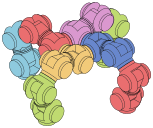
\includegraphics[width=\textwidth]{figures/spider_example.pdf}
        \caption{Walker Robot}
        \label{fig:example_spider}
    \end{subfigure}

    \caption{Examples of metamorphic systems for the case studies.}
\end{figure}

\subsection{Loop Robot}

In the first case study, I would like to first replicate the experiments
performed by \textcite{superbotroller} and
\textcite{DBLP:journals/ijrr/SastraCY09} on the RoFI platform. In their
experiments, they use a loop robot to roll forward (see Figure
\ref{fig:example_roller} for an example of such robot).

\textcite{superbotroller} perform two experiments on loop rolling: the first one
without any communication between modules (the modules act purely based on
observations from their accelerometers) and the second one with a centralized
controller, where the master module controls the other modules.

\textcite{DBLP:journals/ijrr/SastraCY09} perform a centrally controlled
experiment on loop rolling. They leverage the dynamics of the system to move
faster compared to previous work. The controller uses accelerometers in the
modules as feedback.

Once I replicate the experiments, I would like to extend or redesign the
controllers developed by the authors. Overall goal of the redesign is to explore
the problem of fault-tolerance on well-defined case a possibly find a concept of
control worth generalizing to an arbitrary configuration. I plan to introduce
the following improvements:
\begin{itemize}
    \item I will transform the controller into a distributed one as the first
    step towards fault tolerance. This presents mainly a challenge in
    synchronization and information exchange -- especially sensor feedback. We
    would like to include inertial measurements units, obstacle distance and
    torque feedback from the servomotors.
    \item Then I would like to remove the assumption, that the individual
    modules report correct feedback. The controller should be able to deal with
    some number of units that provide incorrect feedback.
    \item If applicable, the controller should also be able to deal with some
    number of units that have faulty joints.
    \item RoFI modules have a joint in the middle, therefore, I will implement
    steering so the loop can turn left and right during motion.
\end{itemize}

There are two ways to tackle the challenges given above. The first,
straigtforward one one and probably easier to handle is to use leader-election
\cite{baca2016coordination} to elect a leading module. Then the system will
monitor whether the leaders is alive and if not, it will reelect a new one. The
leader can centrally collect sensor data and basically remotely control the
other modules. In this case, faulty sensor could be handled in a byzantine way
(e.g., by an approach inspired by \textcite{DBLP:conf/osdi/CastroL99}).

The second approach is to use digital hormones (inspired by
\cite{DBLP:conf/cec/HamannSSC10, DBLP:conf/icra/MorenoG11}) for both, control
and sensor feedback. This approach is more appealing as it leverages the basics
of the self-reconfigurable robots and possible, should yield better results and
inherently tackle both sensors and actuators faults. However, as
literature shows, it is hard to apply.

Nevertheless, in both approaches, we would like to leverage the dynamics of the
system to move faster and to be able to steer. Suitable inspiration could be
taken from cable robots, which often resemble the configuration used in this
case study and thus, deal with similar problems in locomotion
\cite{DBLP:conf/iros/Hustig-SchultzS16, DBLP:conf/iros/CeraA18}. If we manage to
distribute sensor feedback well, it could open a possibility for the loop to
roll on bumpy terrain or stairs.

\subsection{Walker Robot}

The second case study should directly built on the results of the first one. My
goal is to take a non-trivial configuration (e.g., walker in Figure
\ref{fig:example_spider}) and apply my findings on it to perform synchronous
execution of a movement yielding locomotion by walking on a flat surface. The
goal of this study is to help me find generalizable approaches for control.

If we use the leader-election approach, this case study will focus on efficiency
of communication and scalability to large systems possibly by introducing a
hierarchical approach (i.e., there is a separate leader for each limb of the
robot and synchronization is only required among limb leaders and among modules
belonging to the same limb).

If we use the hormone-based approach, this case study will probably focus on
designing suitable hormone system for such configurations. We could explore the
possibility of introducing a library of hormone primitives that could be
composed together and thus simplify design of complex hormone-based controllers.

\section{Time Plan}

The plan of my future study and research activities is following:

\begin{description}[style=nextline,leftmargin=0.8cm]
    \item [now -- January 2023]
        Development and maintenance of the RoFI platform.
    \item [now -- January 2021]
        Replication of the loop robot experiments for RoFI.
    \item [January 2021]
        Doctoral exam and defense of this thesis proposal.
    \item [February 2021 -- June 2021]
        Designing the new controller for the loop configuration and
        investigation of fault-tolerant approaches.
    \item [June 2021 -- December 2022]
        Generalization of the outcomes of the loop configuration case study.
    \item[January 2022 -- August 2022]
        Application of the findings in context of complex configurations.
    \item[September 2022 -- January 2023]
        Summarizing my research and writing of the PhD thesis.
    \item[January 2023]
        Defense of the PhD thesis.
\end{description}
